\documentclass[12pt,a4paper]{article}
% 文档类:12pt字体,A4纸张,文章类型
\usepackage[margin=1in]{geometry}
% 几何包:设置1英寸边距
\usepackage{graphicx}
% 图形包:插入图片
\usepackage{amsmath}
% AMS数学包:数学公式
\usepackage{amssymb}
% AMS符号包:数学符号
\usepackage{newtxtext,newtxmath} % Times New Roman 字体
% New TX字体包:Times New Roman字体
\usepackage{setspace} % 行距设置
% Setspace包:行距设置
\usepackage{siunitx}
% SI单位包:科学单位
\usepackage[hidelinks]{hyperref} % 去除目录/链接红框
\usepackage[backend=biber, style=ieee]{biblatex}
\addbibresource{references.bib}
% Hyperref包:超链接,隐藏链接边框
\usepackage{enumitem}
% Enumitem包:列表项
\usepackage{float}
% Float包:浮动环境
\usepackage{subcaption}
% Subcaption包:子标题


% 设置页面格式:1英寸边距,1.5倍行距,12点Times New Roman字体
\geometry{margin=1in}
\onehalfspacing
\setlength{\parindent}{0pt}
\setlength{\parskip}{6pt}

\title{\textbf{EE5112: Human Robot Interaction\\Project 1: Dialogue System and LLM Platform Development}}
% 标题:EE5112:人机交互\\项目1:对话系统和LLM平台开发
\author{Group 7\\
Niu Mu (Matriculation Number)\\
Wu Zining (A0294373W)\\
Zhao Jinqiu (Matriculation Number)}
\date{\today}
% 日期:今天

\begin{document}
% 文档开始

\maketitle
% 生成标题页

% 标题页
% Title page with group information and course details

\newpage
% 新页

\tableofcontents
% 生成目录

\newpage
% 新页

% 目录
% Table of contents

\section{Abstract}
% 摘要

% 摘要部分 - 简要概述项目目标、方法、主要发现和结论
% Abstract section - Brief overview of project objectives, methods, key findings and conclusions

[Placeholder for abstract content - 150-250 words]
% [摘要内容占位符 - 150-250字]

% 关键词
% Keywords
\textbf{Keywords:} Dialogue System, LLM, Human-Robot Interaction, Natural Language Processing, TensorFlow
% 关键词:对话系统,LLM,人机交互,自然语言处理,TensorFlow

\section{Introduction}
% 引言

% 引言部分 - 介绍对话系统和LLM的背景,项目目标和意义
% Introduction section - Background of dialogue systems and LLMs, project objectives and significance

\subsection{Background}
% 背景

% 背景介绍 - 对话系统在人机交互中的重要性
% Background introduction - Importance of dialogue systems in human-robot interaction

[Placeholder for background content]
% [背景内容占位符]

\subsection{Project Objectives}
% 项目目标

% 项目目标 - 基于课程要求的具体目标
% Project objectives - Specific objectives based on course requirements

The main objectives of this project are:
% 本项目的主要目标是:
\begin{enumerate}
    \item To familiarize with the process of developing a dialogue system
    % 熟悉对话系统开发过程
    \item To familiarize with the working environment and Python packages
    % 熟悉工作环境和Python包
    \item To familiarize with popular platforms such as TensorFlow
    % 熟悉TensorFlow等流行平台
    \item To familiarize with popular open source LLMs (Llama, GLM, etc.)
    % 熟悉Llama、GLM等流行开源LLM
    \item To develop a dialogue system and local LLM platform
    % 开发对话系统和本地LLM平台
    \item To familiarize with LLM evaluation procedures
    % 熟悉LLM评估程序
    \item To provide practical experience in problem-finding and problem-solving
    % 提供问题发现和解决的实践经验
\end{enumerate}


% Task1 
\section{Task 1: Develop the Dialogue Systems according to aspiration/interest.}

% Task2
\section{Task 2: Develop Local Dialogue Systems by Using Open-Source LLMs}

\subsection{Literature Review on Different Categories of LLMs}
% 不同类型LLM的文献综述

Large Language Models (LLMs) can be broadly categorized into three main architectures based on their use of the transformer mechanism \cite{vaswani2017attention}: Encoder-Decoder, Encoder-Only, and Decoder-Only. Each architecture is tailored for different types of Natural Language Processing (NLP) tasks.
% 大型语言模型(LLM)可根据其对Transformer机制的使用情况\cite{vaswani2017attention},大致分为三种主要架构:编码器-解码器、仅编码器和仅解码器。每种架构都针对不同类型的自然语言处理(NLP)任务进行了优化。

\begin{itemize}
    \item \textbf{Encoder-Decoder models}, such as T5 \cite{raffel2020exploring} and BART \cite{lewis2019bart}, utilize both a bidirectional encoder to process the input text and an autoregressive decoder to generate output. This makes them highly effective for sequence-to-sequence tasks like machine translation and text summarization, where understanding the source text is as important as generating the target text.
    % \textbf{编码器-解码器模型},如T5 \cite{raffel2020exploring}和BART \cite{lewis2019bart},同时使用双向编码器处理输入文本和自回归解码器生成输出。这使得它们在机器翻译和文本摘要等序列到序列任务中非常有效,因为在这些任务中,理解源文本与生成目标文本同样重要。
    \item \textbf{Encoder-Only models}, like BERT \cite{devlin2018bert} and RoBERTa \cite{liu2019roberta}, use only the bidirectional encoder. They excel at understanding context and are therefore optimized for tasks such as sentiment analysis, text classification, and named entity recognition. However, they are not inherently suited for text generation.
    % \textbf{仅编码器模型},如BERT \cite{devlin2018bert}和RoBERTa \cite{liu2019roberta},仅使用双向编码器。它们擅长理解上下文,因此针对情感分析、文本分类和命名实体识别等任务进行了优化。然而,它们本身不适合文本生成。
    \item \textbf{Decoder-Only models}, including the GPT series \cite{radford2018improving} and LLaMA \cite{touvron2023llama}, employ a unidirectional (causal) decoder. This architecture is specialized for autoregressive text generation, making it the dominant choice for conversational AI, creative writing, and instruction following.
    % \textbf{仅解码器模型},包括GPT系列 \cite{radford2018improving}和LLaMA \cite{touvron2023llama},采用单向(因果)解码器。该架构专门用于自回归文本生成,使其成为对话AI、创意写作和指令遵循的主流选择。
\end{itemize}

The key differences, performance trade-offs, and typical applications of these architectures are summarized in Table~\ref{tab:llm_comparison}. Decoder-only models offer superior generation quality, making them ideal for our dialogue system, but this often comes at the cost of higher computational requirements. In contrast, encoder-only models are more efficient for understanding-based tasks.
% 这些架构的关键差异、性能权衡和典型应用总结在表~\ref{tab:llm_comparison}中。仅解码器模型提供卓越的生成质量,使其成为我们对话系统的理想选择,但这通常以更高的计算要求为代价。相比之下,仅编码器模型在基于理解的任务上更高效。

\begin{table}[H]
\centering
\caption{Comparison of LLM Architecture Types}
% LLM架构类型比较
\label{tab:llm_comparison}
\begin{tabular}{|l|l|l|l|}
\hline
\textbf{Aspect} & \textbf{Encoder-Decoder} & \textbf{Encoder-Only} & \textbf{Decoder-Only} \\
% 方面 & 编码器-解码器 & 仅编码器 & 仅解码器
\hline
Primary Use & Seq2Seq tasks & Understanding tasks & Generation tasks \\
% 主要用途 & Seq2Seq任务 & 理解任务 & 生成任务
\hline
Attention & Bidirectional + Causal & Bidirectional & Causal \\
% 注意力机制 & 双向 + 因果 & 双向 & 因果
\hline
Task Flexibility & High & Medium & High \\
% 任务灵活性 & 高 & 中等 & 高
\hline
Representative Models & T5, BART & BERT, RoBERTa & GPT, LLaMA \\
% 代表性模型 & T5, BART & BERT, RoBERTa & GPT, LLaMA
\hline
\end{tabular}
\end{table}

Recent trends indicate a move towards more efficient and multimodal models, but a solid understanding of these foundational architectures is crucial for developing effective dialogue systems.
% 最近的趋势表明,模型正朝着更高效和多模态的方向发展,但对这些基础架构的深入理解对于开发有效的对话系统至关重要。

% 对不同LLM架构的全面理解为在对话系统和本地LLM平台中选择适当模型提供了基础。




% Task 2.2
\subsection{Local LLM Platform Implementation}

We deploy a compact local dialogue stack around the quantized \texttt{Llama-3.2-3B-Instruct-Q4\_K\_M.gguf} checkpoint to provide offline interaction without sacrificing responsiveness.
% 部署基于量化 Llama-3.2-3B-Instruct-Q4_K_M.gguf 的轻量本地对话栈,实现离线交互并保持响应速度

\noindent\textbf{Architecture.} \texttt{llm\_platform.py} wraps \texttt{llama-cpp-python} for model loading and inference, while \texttt{dialogue\_system.py} manages the chat loop, prompt templating, streaming output, and defensive error handling. The separation keeps model plumbing isolated from user interaction logic.
% 架构层面将模型加载推理与对话管理解耦,llm_platform.py 负责底层推理,dialogue_system.py 负责交互与容错

\noindent\textbf{Inference pipeline.} Configuration values expose only the essentials: a 4,096-token context window, generation controls (temperature and maximum new tokens), and an optional GPU layer count for acceleration. Switching between CPU and CUDA execution is done in \texttt{config.json} without touching the code base.
% 推理流程仅暴露上下文长度、采样控制和 GPU 层数等核心参数,可在 config.json 中无缝切换 CPU/GPU

\noindent\textbf{User experience and persistence.} The terminal interface streams tokens as they are produced, retains up to six dialogue turns, supports maintenance commands (\texttt{exit}/\texttt{clear}/\texttt{stats}), and records each session as ISO8601-stamped JSON under \texttt{conversations/} for later auditing.
% 终端界面支持流式输出、保留最多六轮上下文,提供退出/清除/统计命令,并以 ISO8601 时间戳保存会话记录

\noindent\textbf{Portability.} The same stack runs on laptops or desktop GPUs, making it suitable for privacy-sensitive deployments and quick benchmarking. Figure~\ref{fig:llama_cpu_chat} illustrates the interface operating in CPU mode.
% 该方案可在笔记本或桌面 GPU 上部署,兼顾隐私场景与快速评测,图~\ref{fig:llama_cpu_chat} 展示其 CPU 模式界面

\begin{figure}[H]
    \centering
    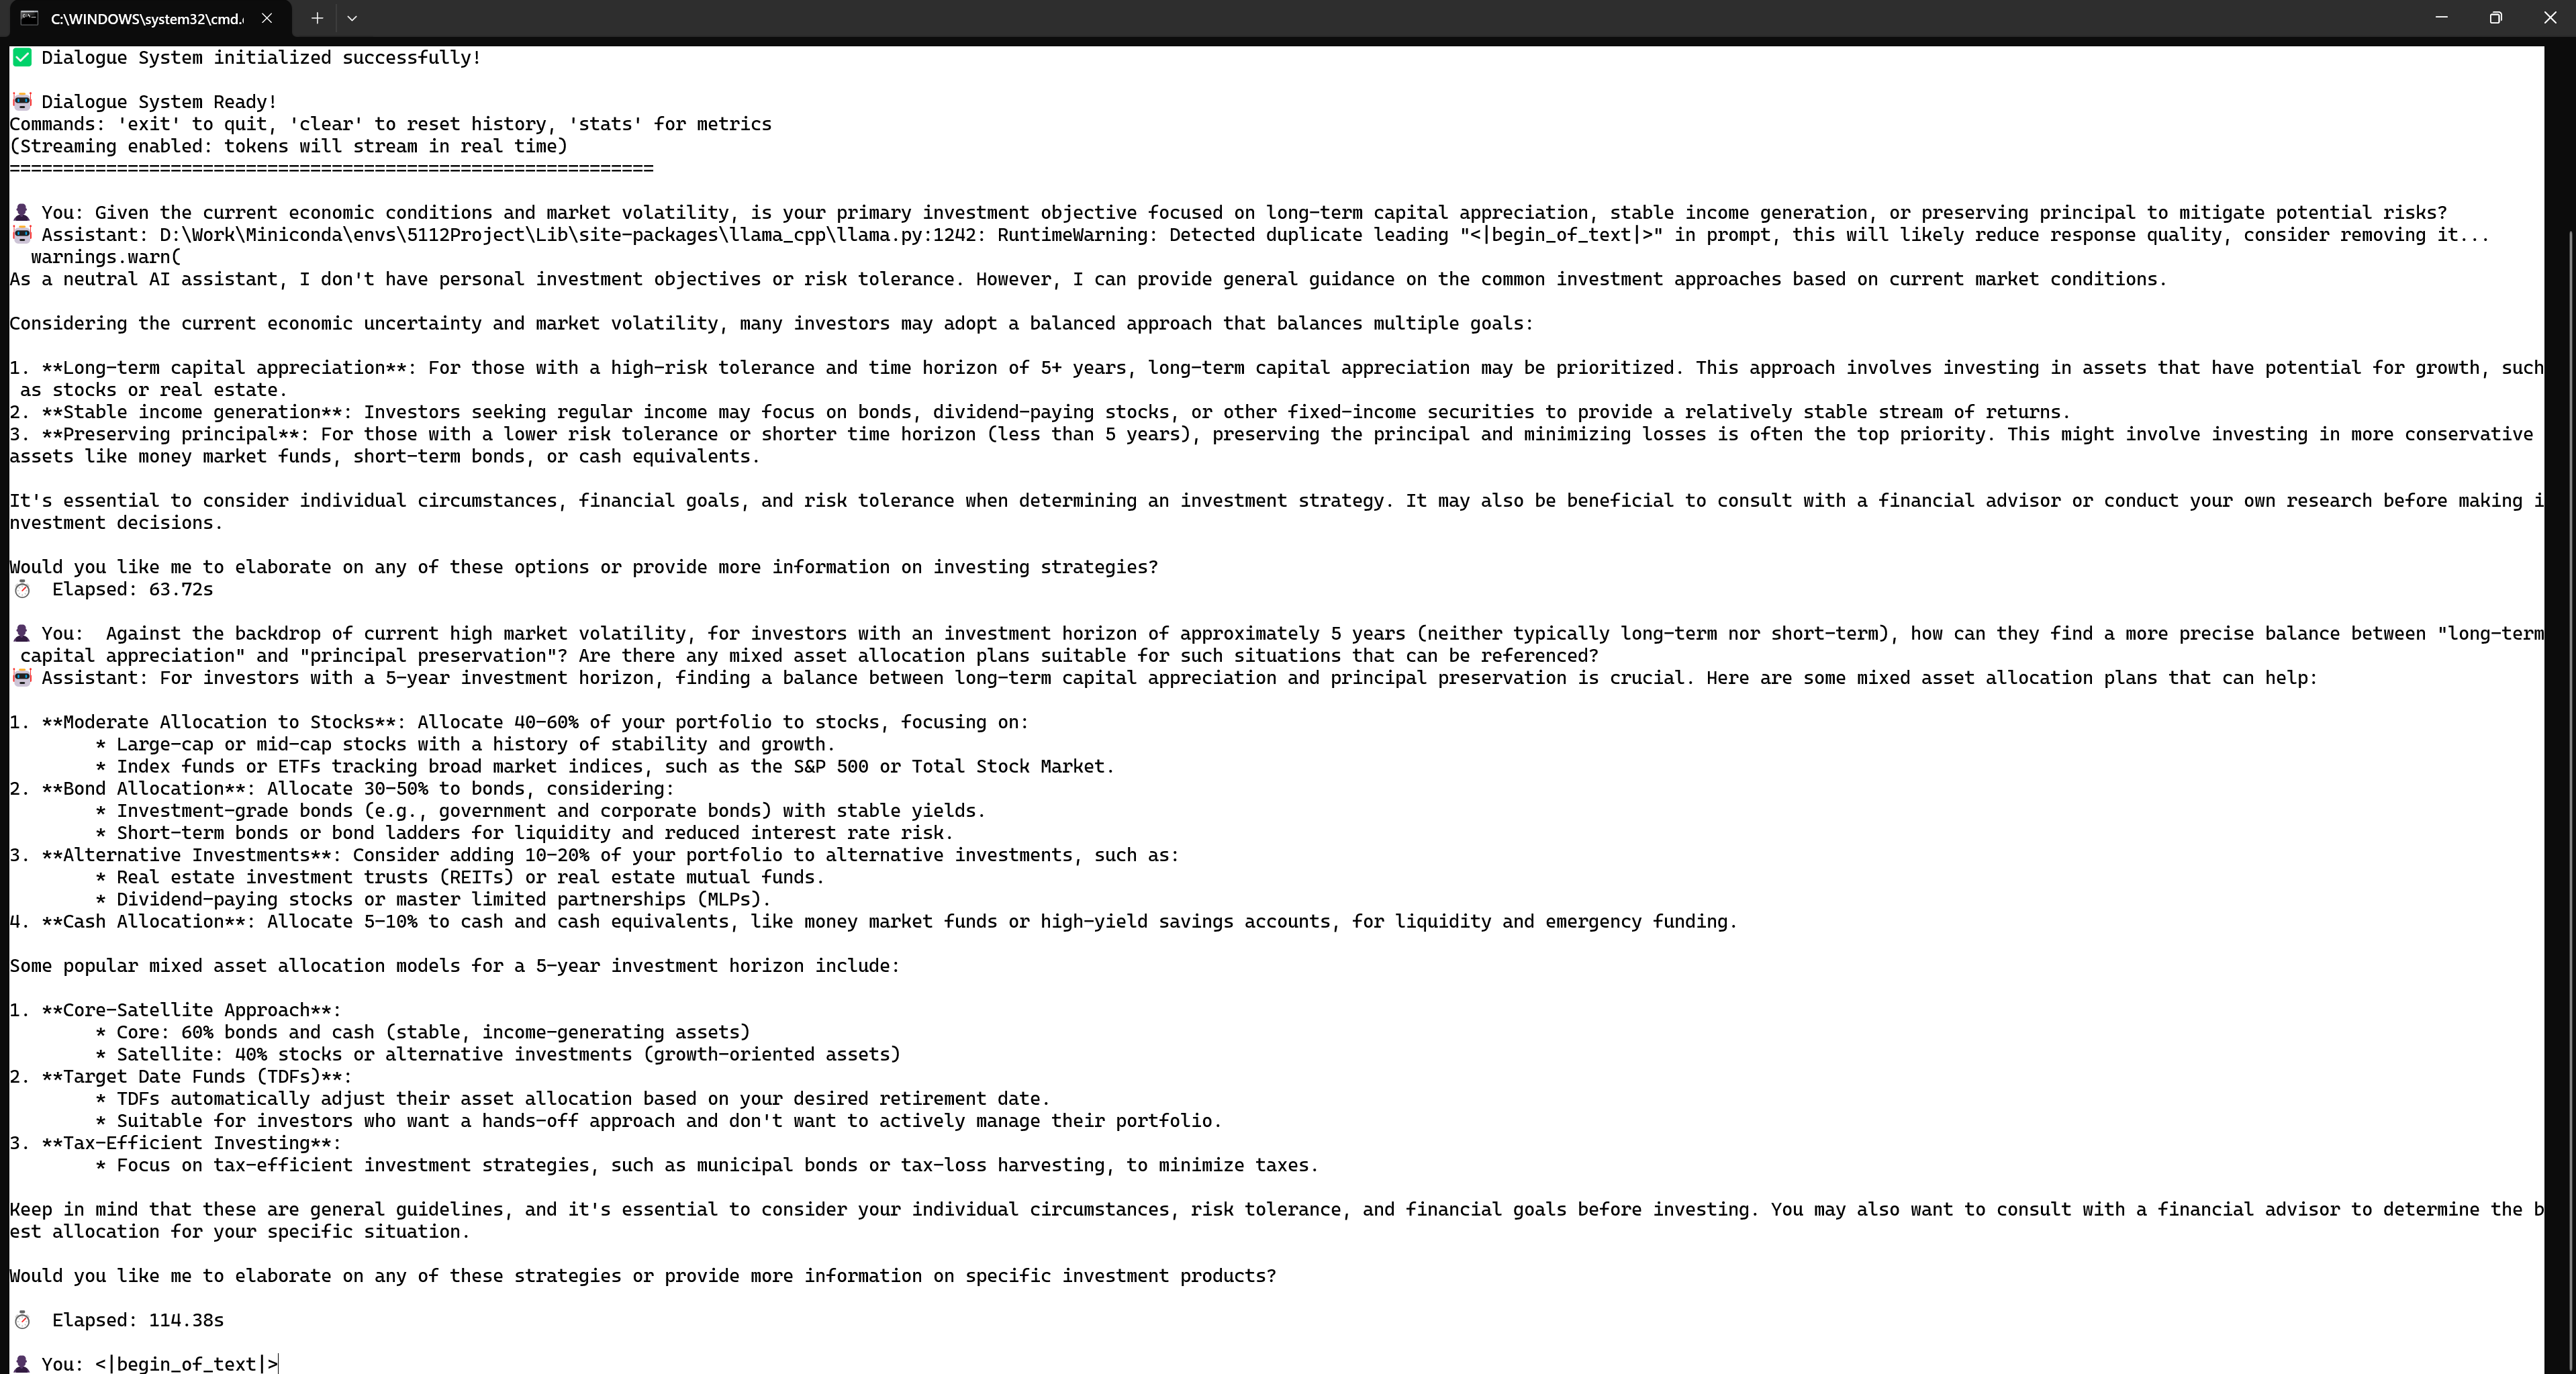
\includegraphics[width=0.95\linewidth]{Figures/llama对话.png}
    \caption{Terminal-based dialogue interface showing multi-turn conversation capabilities}
    \label{fig:llama_cpu_chat}
\end{figure}





\subsection{Performance Comparison: CPU vs GPU Deployment}
% 性能比较:CPU 与 GPU 部署

To quantify the benefit of the dedicated GPU pipeline, we benchmarked identical prompts (	extit{"hello"} and 	extit{"Who are you?"}) on both deployment targets using the same quantized \texttt{Llama-3.2-3B-Instruct-Q4\_K\_M.gguf} model and configuration. Timing was captured end-to-end from user input to the final token, with streaming enabled in both runs. The GPU test was executed on an RTX 5080 16GB with cuBLAS acceleration, whereas the CPU baseline was collected on the same workstation with GPU offloading disabled.
% 为量化 GPU 管线带来的收益,我们在 CPU 与 GPU 上使用相同提示词和同一量化模型进行基准测试,记录从输入到生成完成的端到端耗时。

\begin{table}[H]
    \centering
    \caption{Inference latency comparison between CPU and GPU backends}
    % CPU 与 GPU 推理延迟比较
    \label{tab:cpu_gpu_latency}
    \begin{tabular}{|l|c|c|c|}
        \hline
        	extbf{Prompt} & \textbf{CPU latency (s)} & \textbf{GPU latency (s)} & \textbf{Speedup} \\
        % 提示词 & CPU 延迟 & GPU 延迟 & 加速比
        \hline
        hello & 4.90 & 2.44 & 2.0\texttimes{} \\
        Who are you? & 22.40 & 11.18 & 2.0\texttimes{} \\
        \hline
    \end{tabular}
\end{table}

Across both prompts, the GPU path halves the response time while preserving output quality. The reduction primarily stems from mapping transformer layers onto CUDA kernels (\texttt{n\_gpu\_layers = -1}) via \texttt{llama-cpp-python} with \texttt{LLAMA\_CUBLAS=1}, eliminating the CPU bottleneck observed in the baseline. Shorter latency also improves conversational fluidity because streamed tokens begin appearing almost immediately, keeping the user engaged.
% GPU 方案将耗时缩短约一半,主要得益于使用 cuBLAS 将 transformer 层映射到 GPU,从而消除 CPU 瓶颈。

Figure~\ref{fig:llama_cpu_chat} shows the slower CPU baseline, while Figure~\ref{fig:llama_gpu_chat} captures the accelerated GPU session that produced the timings in Table~\ref{tab:cpu_gpu_latency}.
% 图~\ref{fig:llama_cpu_chat} 展示 CPU 基线,图~\ref{fig:llama_gpu_chat} 对应 GPU 加速会话。

\begin{figure}[H]
    \centering
    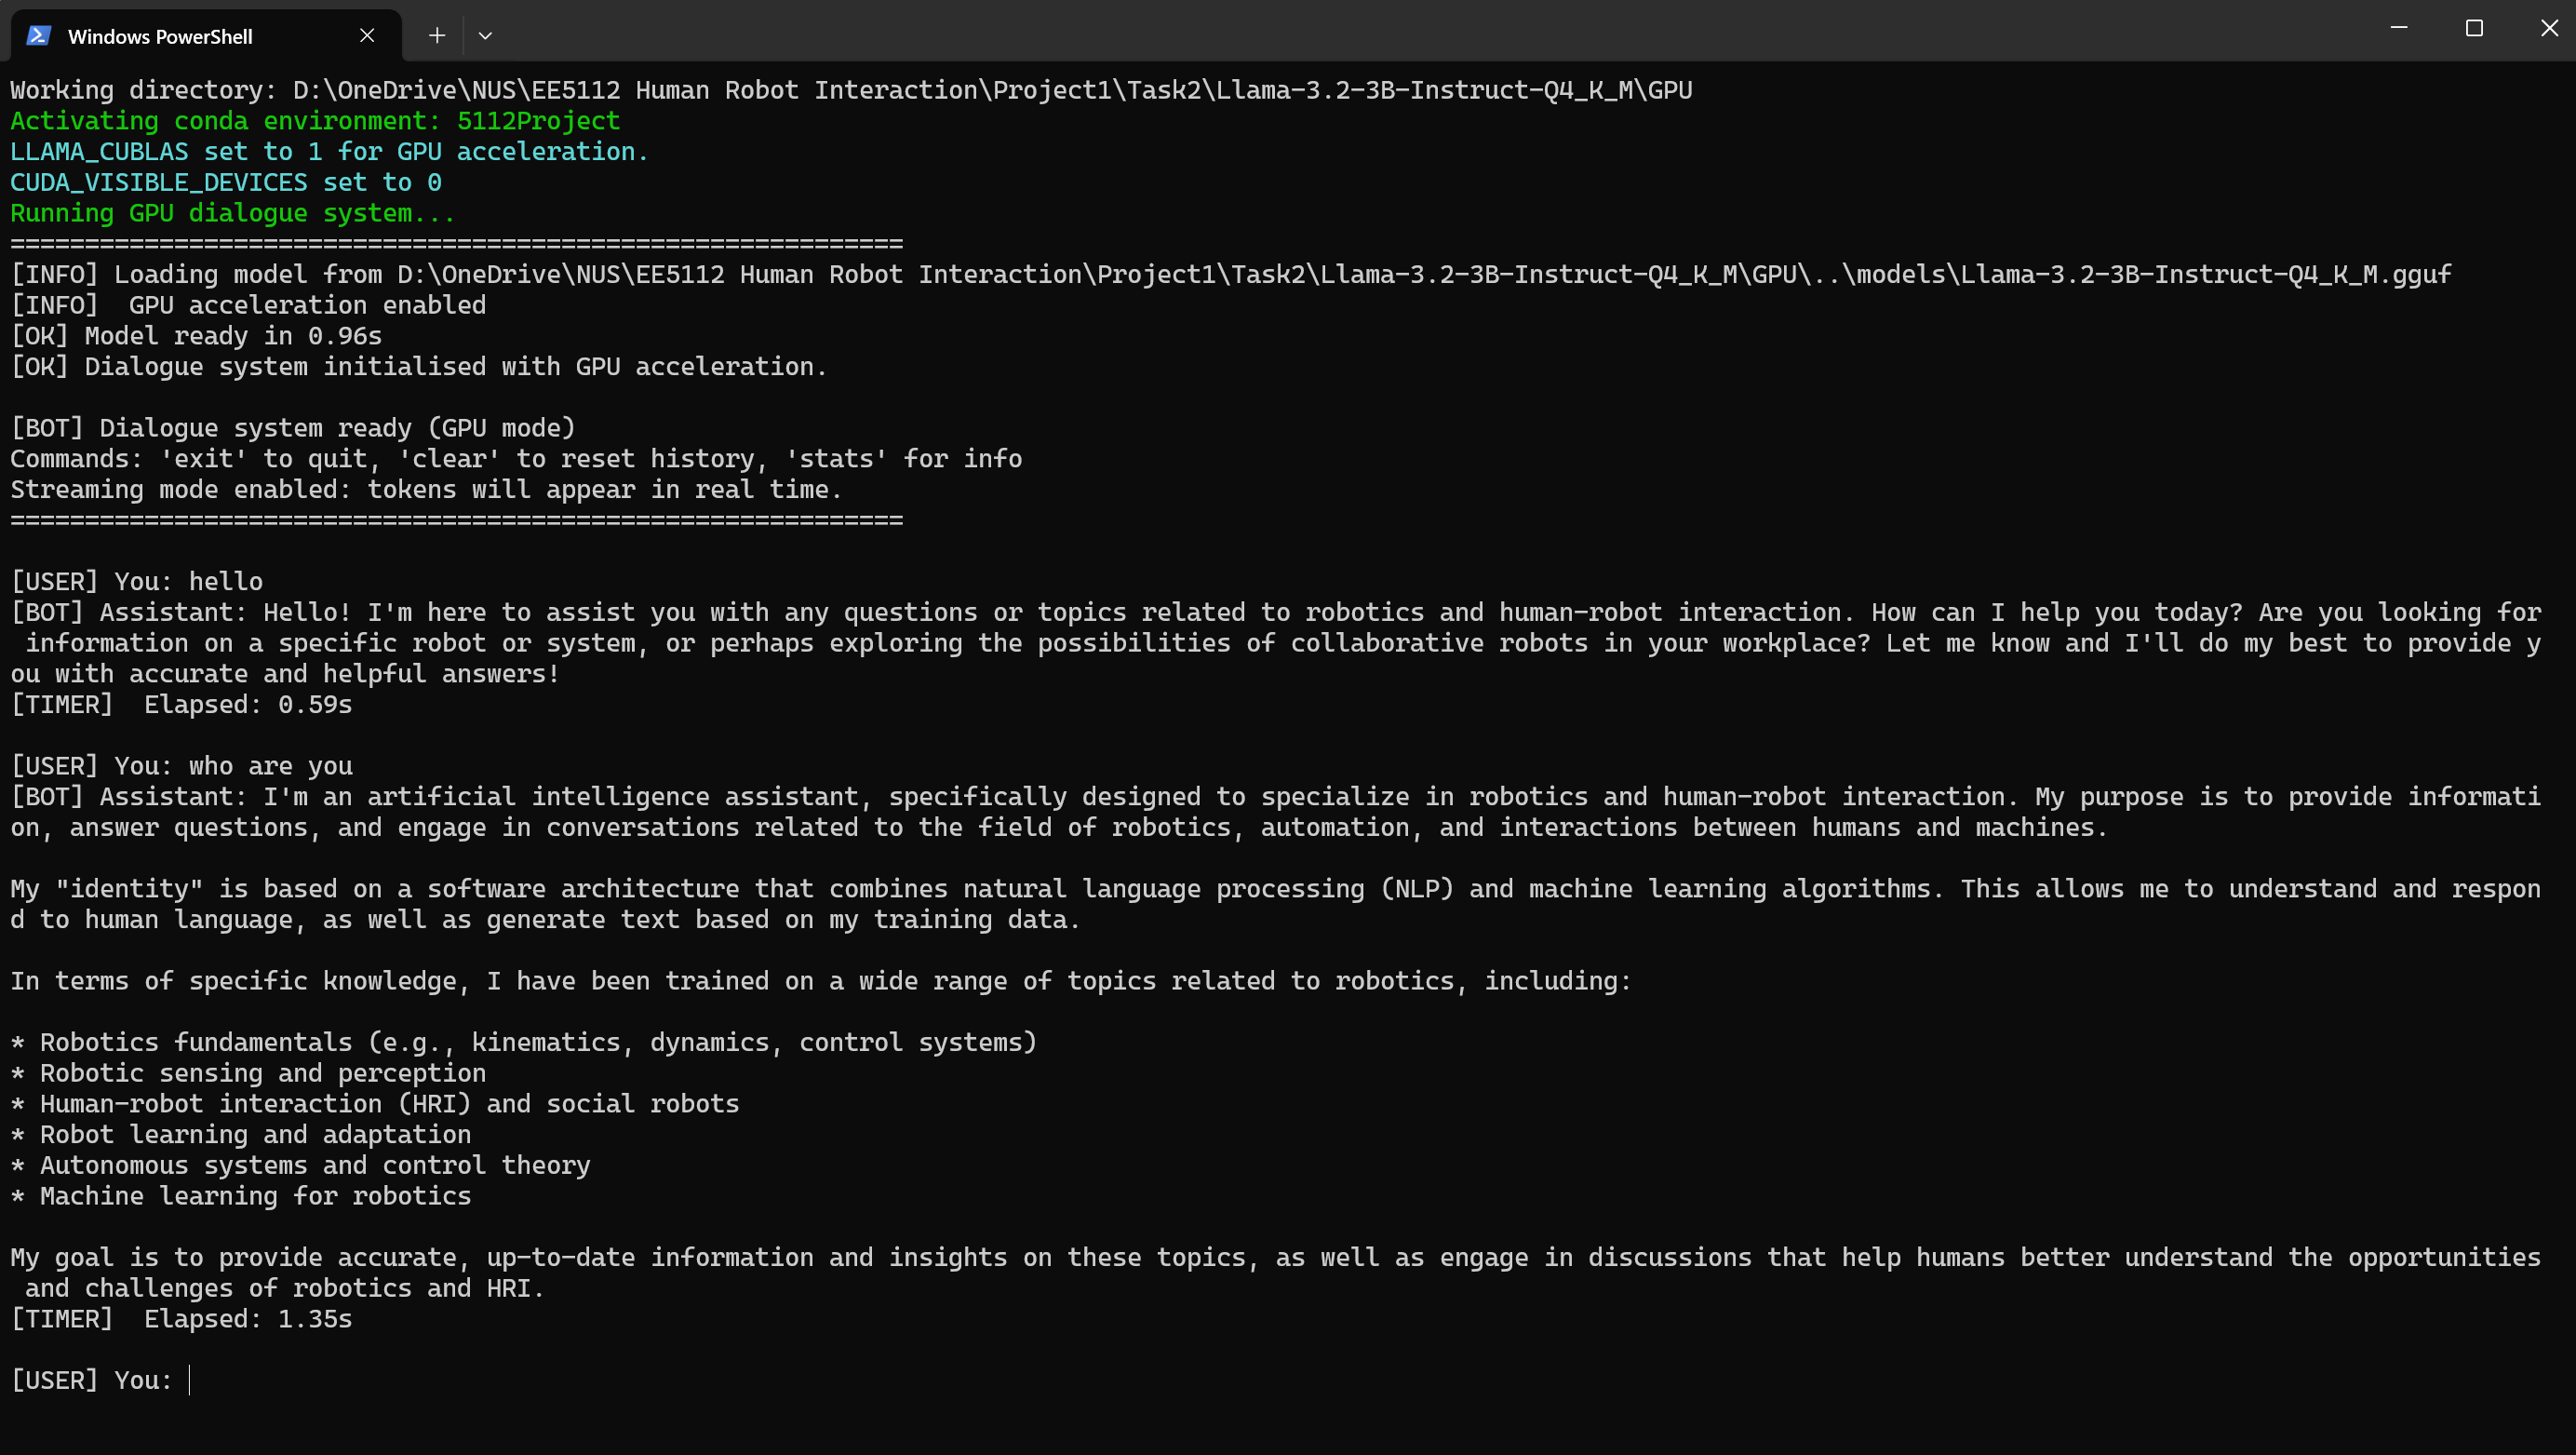
\includegraphics[width=1\linewidth]{Figures/llamaGPU.png}
    \caption{Streaming dialogue captured during the GPU benchmark run.}
    % GPU 基准运行时捕获的流式对话截图
    \label{fig:llama_gpu_chat}
\end{figure}

\subsection{Comparation of Different Pretrained Models}
% 不同预训练模型的比较

\subsection{Challenges in Deployment}

While experimenting with the full-size Llama-3.1-8B-Instruct checkpoint, we encountered practical constraints on the RTX 5080 (16 GiB). Model weights alone consumed roughly 15.4 GiB in FP16, leaving little headroom for KV caches and activations. Consequently, the system frequently raised CUDA out-of-memory errors even before completing a single response.
% 在 RTX 5080(16 GiB)上加载 Llama-3.1-8B Instruct 时,FP16 权重占用约 15.4 GiB 显存,几乎没有空间留给 KV 缓存与中间激活,导致推理尚未完成就频繁触发 CUDA OOM。

We mitigated the tokenizer crash by forcing \texttt{TOKENIZERS\_PARALLELISM=false} and limiting \texttt{RAYON\_NUM\_THREADS}. However, memory pressure remained the dominant bottleneck. Even aggressive limits on \texttt{max\_new\_tokens} and history length provided only marginal relief, so conversations still terminated abruptly once GPU memory fragmented.
% 通过设置 TOKENIZERS_PARALLELISM=false 和 RAYON_NUM_THREADS 等环境变量,解决了分词线程池崩溃问题,但显存压力仍是主要瓶颈;即便收紧 max_new_tokens 与历史长度,OOM 依旧发生。

Given the strict memory ceiling and unstable experience, we migrated the local deployment to the quantized Llama-3.2-3B-Instruct-Q4\_K\_M model. It delivers comparable interaction quality while fitting comfortably within both GPU and CPU budgets.
% 鉴于显存限制和交互不稳定,我们最终采用量化的 Llama-3.2-3B-Instruct-Q4_K_M 替代方案,在 GPU 与 CPU 环境下都能稳定运行并保持近似的对话质量。


% Task3
\section{Task 3: LLM Performance Evaluation}
% 任务3:LLM性能评估

[Placeholder for Task 3 content]
% [任务3内容占位符]

% Task4
\section{Task 4: GUI for Local LLM}
% 任务4:为本地LLM设计图形用户界面(GUI)

[Placeholder for Task 4 content]
% [任务4内容占位符]

% Task5
\section{Task 5: Exploring Multimodal Large Language Models (MLLMs)}
% 任务5:探索多模态大型语言模型(MLLMs)

[Placeholder for Task 5 content]
% [任务5内容占位符]


\subsection{Solution Implementation}
% 解决方案实现

% 解决方案实现 - 针对挑战的具体解决方案
% Solution implementation - Specific solutions to challenges

[Placeholder for solution implementation content]
% [解决方案实现内容占位符]

\subsection{Code Documentation}
% 代码文档

% 代码文档 - 项目代码的文档化
% Code documentation - Documentation of project code

[Placeholder for code documentation content]
% [代码文档内容占位符]

\section{Results and Discussion}
% 结果和讨论

% 结果和讨论 - 对项目成果的深入讨论和分析
% Results and discussion - In-depth discussion and analysis of project outcomes

\subsection{System Performance Results}
% 系统性能结果

% 系统性能结果 - 展示系统测试结果
% System performance results - Present system testing results

[Placeholder for system performance results content]
% [系统性能结果内容占位符]

\subsection{Task Achievement Summary}
% 任务完成情况总结

% 任务完成情况总结 - 总结各任务的完成情况
% Task achievement summary - Summary of completion status for each task

[Placeholder for task achievement summary content]
% [任务完成情况总结内容占位符]

\subsection{Lessons Learned}
% 经验教训

% 经验教训 - 从项目中学到的经验
% Lessons learned - Experiences gained from the project

[Placeholder for lessons learned content]
% [经验教训内容占位符]

\section{Individual Contributions}
% 个人贡献

% 个人贡献 - 每个组员的个人贡献说明
% Individual contributions - Individual contribution statements for each group member

\subsection{Member 1: Niu Mu}
% 组员1:牛牧

% 组员1:牛牧 - 个人贡献说明
% Member 1: Niu Mu - Individual contribution statement

[Placeholder for Niu Mu's contributions]
% [牛牧贡献占位符]

\subsection{Member 2: Wu Zining (A0294373W)}
% 组员2:吴子宁

% 组员2:吴子宁 - 个人贡献说明
% Member 2: Wu Zining - Individual contribution statement

[Placeholder for Wu Zining's contributions]
% [吴子宁贡献占位符]

\subsection{Member 3: Zhao Jinqiu}
% 组员3:赵金秋

% 组员3:赵金秋 - 个人贡献说明
% Member 3: Zhao Jinqiu - Individual contribution statement

[Placeholder for Zhao Jinqiu's contributions]
% [赵金秋贡献占位符]

\section{Conclusion}
% 结论

% 结论 - 总结项目成果和贡献
% Conclusion - Summary of project outcomes and contributions

\subsection{Project Objectives Achievement}
% 项目目标达成情况

% 项目目标达成情况 - 总结项目目标的完成情况
% Project objectives achievement - Summary of project objective completion

[Placeholder for project objectives achievement content]
% [项目目标达成情况内容占位符]

\subsection{Future Work}
% 未来工作

% 未来工作 - 可能的改进方向
% Future work - Possible directions for improvement

[Placeholder for future work content]
% [未来工作内容占位符]

\section{References}
% 参考文献

\printbibliography
% 打印参考文献列表

\section{Appendix}
% 附录

% 附录 - 补充材料如代码片段、配置文件等
% Appendix - Supplementary materials such as code snippets, configuration files, etc.

\subsection{Code Documentation}
% 代码文档

% 代码文档 - 主要代码片段的文档
% Code documentation - Documentation of main code snippets

[Placeholder for code documentation]
% [代码文档占位符]

\subsection{Configuration Files}
% 配置文件

% 配置文件 - 系统配置文件
% Configuration files - System configuration files

[Placeholder for configuration files]
% [配置文件占位符]

\subsection{User Manual}
% 用户手册

% 用户手册 - 系统使用说明
% User manual - System usage instructions

[Placeholder for user manual]
% [用户手册占位符]

\end{document}
% 文档结束
